\documentclass{article}
% \usepackage[utf8]{inputenc}
% \usepackage[T1]{fontenc}
\usepackage{graphicx}
\usepackage{amsmath}
\usepackage{amssymb}
\usepackage{hyperref}
\usepackage{listings}
\usepackage{booktabs}
\usepackage{longtable}
% \usepackage{xeCJK}
\usepackage[space]{grffile}
\usepackage{geometry}
\geometry{a4paper, margin=1in}

\title{CUDA Programming Notes (CMPS 297 GPU)}
\author{Combined Notes}
\date{\today}

\begin{document}
\maketitle
\tableofcontents
\newpage
\section{GPU Architecture}

\begin{itemize}
\item Threads are assigned to SMs at block granularity. (All threads in a block are assigned to the same SM.) Each SM has a limited amount of resources.
\item Threads within the same block can collaborate in ways that threads in different blocks cannot:
\begin{itemize}
\item barrier synchronization (e.g., \_\_syncthreads())
\item shared memory
\item others
\end{itemize}
\item Thread scheduling: warp. 32 threads in a warp are scheduled together and executed following a SIMD model.
\begin{itemize}
\item control divergence: branches, loops
\item latency hiding: when some threads are stalled, the SM can switch to another warp that is ready to execute.
\end{itemize}
\item Occupancy constraints

\begin{longtable}{l|l|l|l|l|l|l|l|l|l}
\hline
GPU Name & K40 & M40 & P100 & V100 & A100? & RTX 3090? & RTX 4090? & H100? & RTX 5090? \\ \hline
Microarchitecture & Kepler & Maxwell & Pascal & Volta & Ampere & Ampere & Ada Lovelace & Hopper & Blackwell \\ \hline
Compute Capability & 3.5 & 5.2 & 6.0 & 7.0 & 8.0 & 8.6 & 8.9 & 9.0 & 12.0 \\ \hline
Number of SMs & 15 & 24 & 56 & 80 & 108 & 82 & 128 & 144 & 192 \\ \hline
Cores per SM & 192 & 128 & 64 & 64 & 64 & 64 & 128 & 128 & 128 \\ \hline
Max threads per SM & 2048 & 2048 & 2048 & 2048 & 2048 & 2048 & 2048 & 2048 & 1536 (48 warps) \\ \hline
Max blocks per SM & 16 & 32 & 32 & 32 & 32 & 16 & 32 & 32 & 32 \\ \hline
Max threads per block & 1024 & 1024 & 1024 & 1024 & 1024 & 1024 & 1024 & 1024 & 1024 \\ \hline
Registers per SM & 64K & 64K & 64K & 64K & 64K & 64K & 64K & 64K & 64K \\ \hline
Shared memory per SM & 48KB & 96KB & 64KB & 96KB & 164KB & 128KB & 128KB & 228KB & 256KB \\ \hline
\end{longtable}

\end{itemize}

\newpage
\section{GPU Memory}

(v100 era)


\begin{itemize}
\item performance metrics
\begin{itemize}
\item FLOPS rate; compute-bound
\item memory bandwidth; memory-bound
\end{itemize}
\item Example: matrix multiplication
\begin{itemize}
\item for $N\times N$ matrices
\begin{itemize}
\item Data loaded: $8N^2$ B
\item Operations: $2N^3$ OP
\item potential compute-to-memory ratio: $0.25 N$ OP/B
\end{itemize}
\item opportunity: memory accesses in the kernel code to reuse input data loaded from global memory as much as possible
\end{itemize}
\item memory in GPU
\begin{itemize}
\item global memory: $\approx 500$ cycles
\item L1 cache: $\approx 5$ cycles, managed by hardware
\item shared memory: $\approx 5$ cycles, managed by programmer
\item constant cache: $\approx 5$ cycles, managed by programmer
\item L2 cache
\item registers: $\approx 1$ cycle

\end{itemize}
\end{itemize}
\begin{figure}
\centering
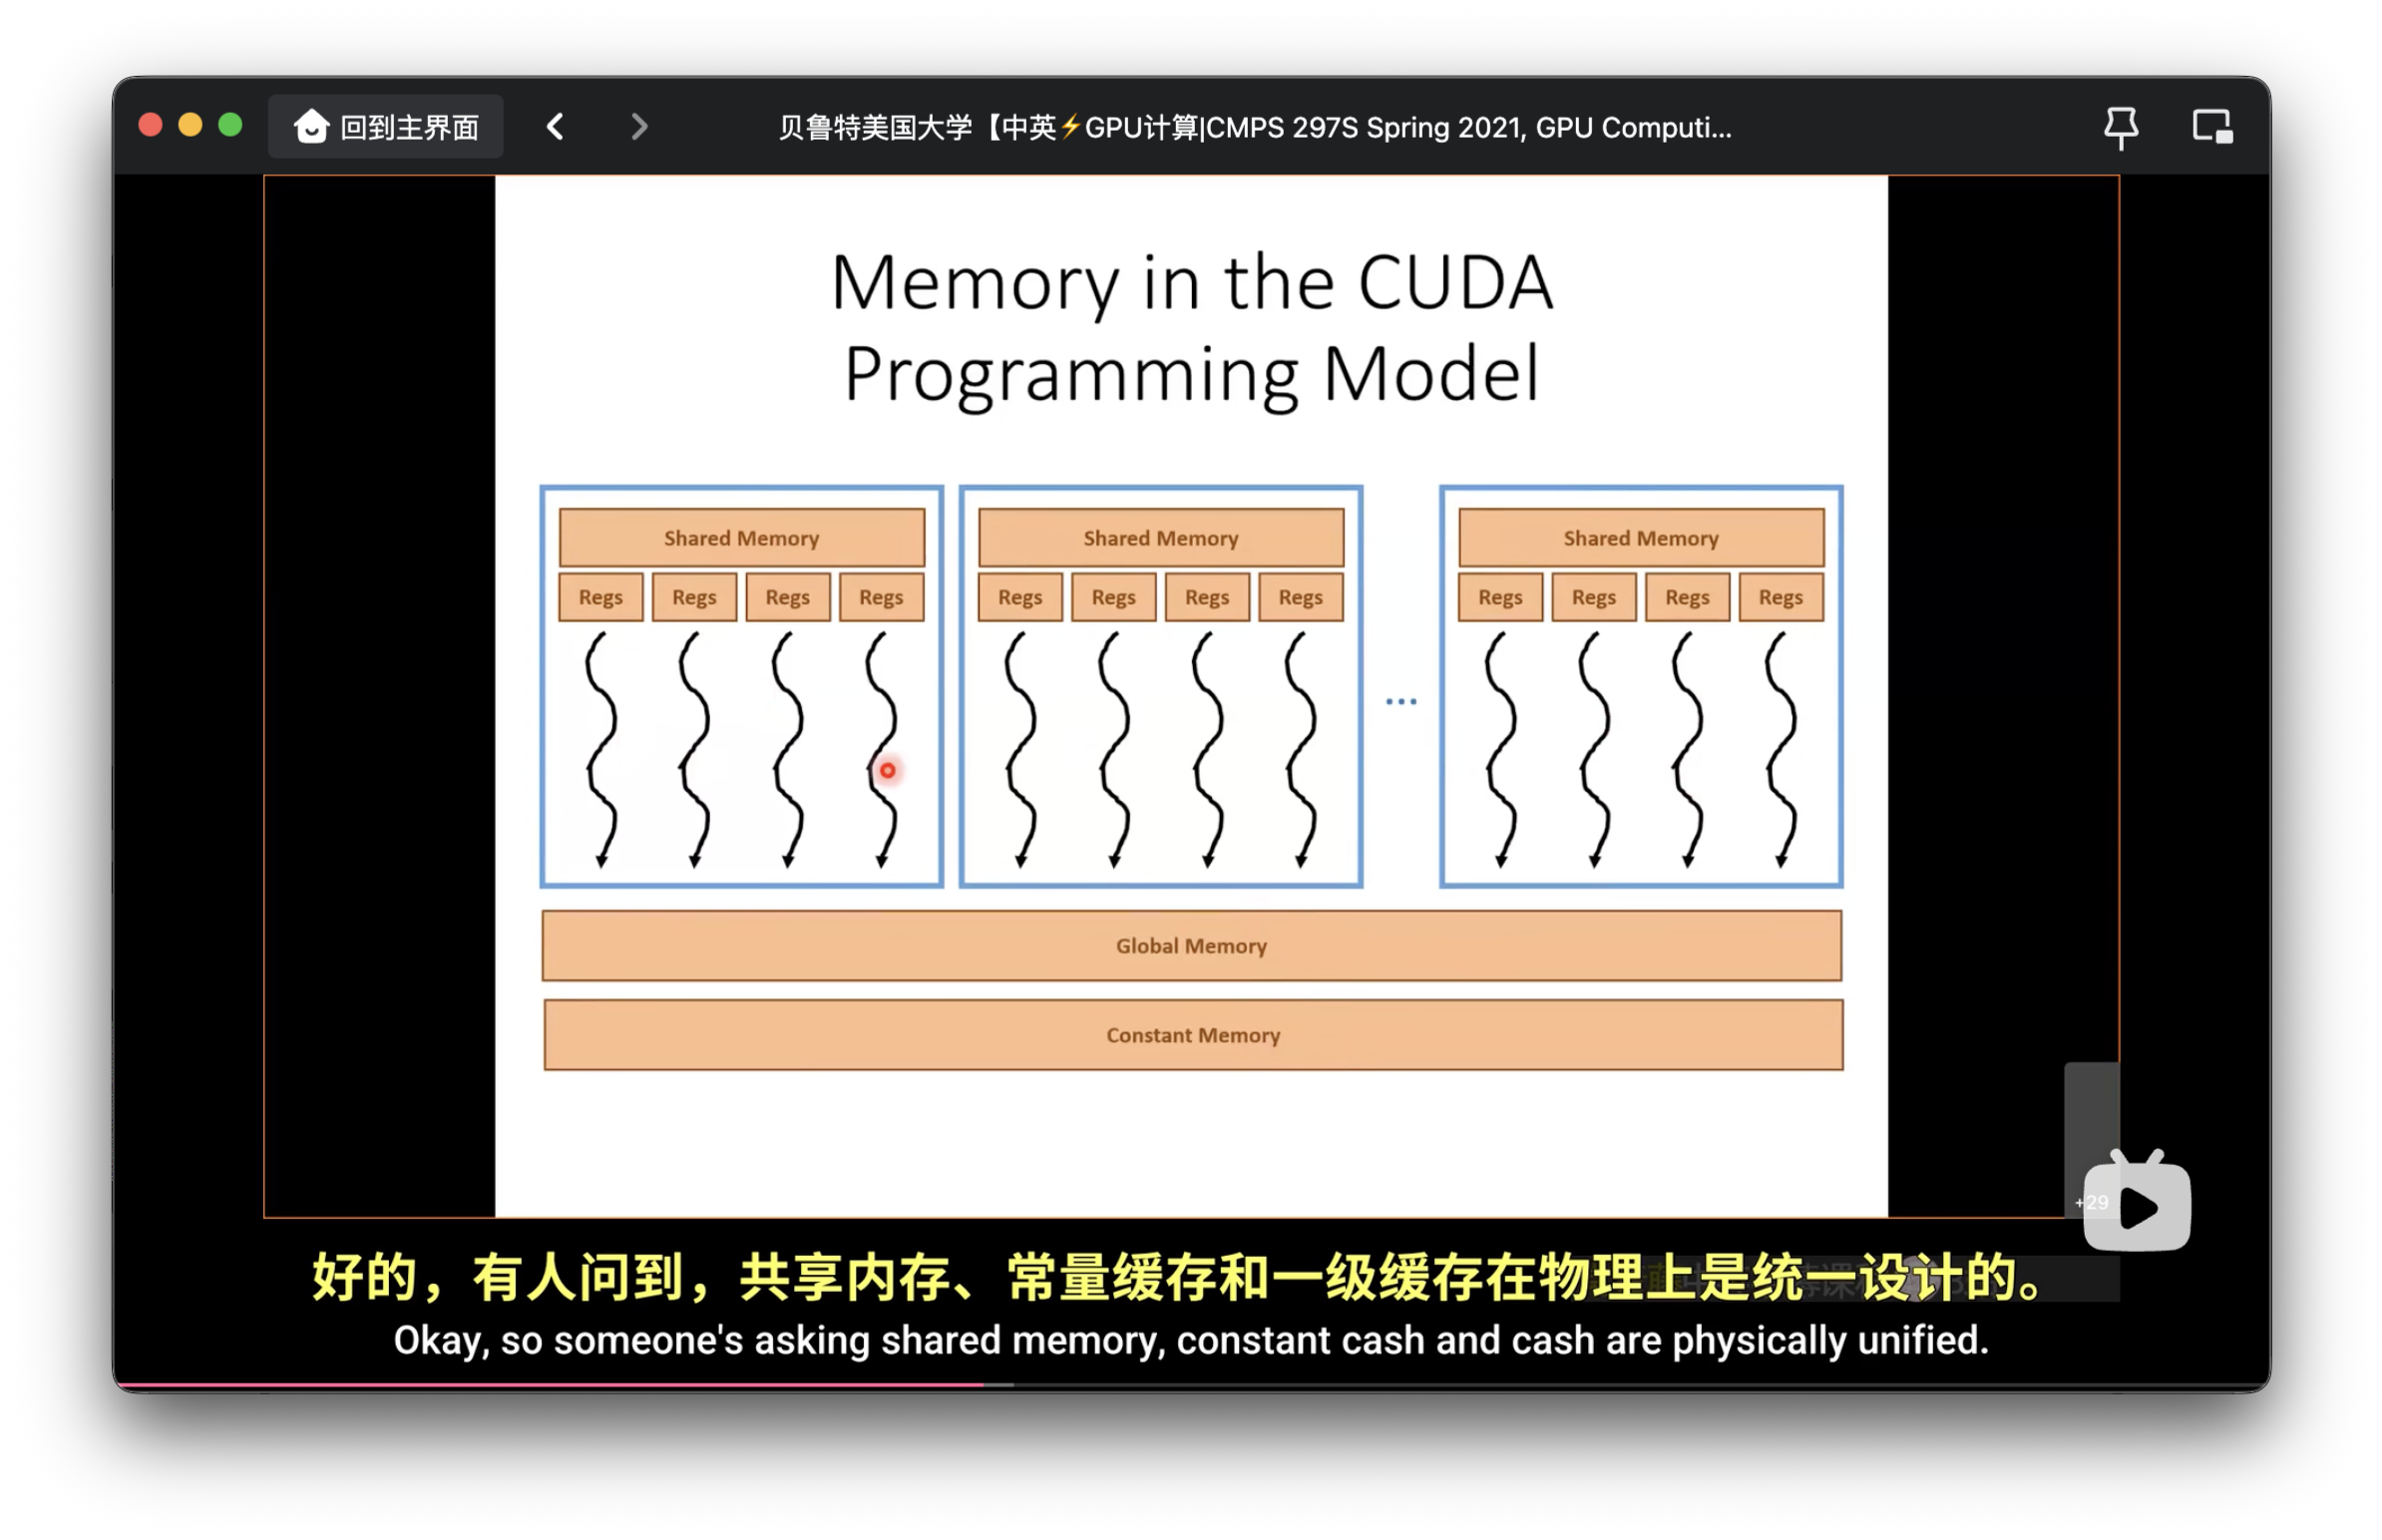
\includegraphics[width=0.8\textwidth]{images/截屏2026-04-28 下午2.16.06.png}
\caption{Memory in the CUDA Programming Model}
\end{figure}
\begin{table}
    \centering
\begin{tabular}{rccc}
\hline
Variable declaration & Memory & Scope & Lifetime \\ \hline
\texttt{\_\_device\_\_ int globalVar;\ \ } & global & grid & application \\
\texttt{\_\_device\_\_ \_\_constant\_\_ int constantVar;} & constant & grid & application \\
\texttt{\_\_device\_\_ \_\_shared\_\_ int sharedVar;\ \ } & shared & block & block \\
\texttt{int localVar;\ \ \ } & register & thread & thread \\
\texttt{int localArr[N];} & global & thread & thread \\ \hline
\end{tabular}
\caption{CUDA Type Qualifiers}
\end{table}
The data gets evicted from the L1 cache before another thread tries to load it, more likely than CPU because of the large number of threads and the small size of the L1 cache.


Dynamic shared memory

\begin{itemize}
\item declaration: \texttt{extern \_\_shared\_\_ float A\_s[];}
\item configuration: \texttt{kernel <<< numBlocks, numThreadsPerBlock, smemPerBlock >>> (...)}
\end{itemize}

\newpage
\section{Performance Metrics}
some Performance Optimizations


\begin{itemize}
\item Tuning resource usage to maximize occupancy
\begin{itemize}
\item Threads per block, shared memory per block, registers per thread [p4]
\end{itemize}
\item Minimizing control divergence to increase SIMD efficiency [p4]
\item Shared memory tiling to increase data reuse [p5]
\item Memory coalescing
\item Thread coarsening

\end{itemize}
DRAM cell: consists of a capacitance that stores a charge and a three-state device (single-transistor) that allows data to be read/written (capacitor discharged/charged).


DRAM array, DRAM bank.


Row Address $\to$ [Row Decoder] $\to$ [DRAM Array] $\to$ [Sense Amplifier] $\to$ [Column Latches] $\xrightarrow{\text{burst}}$ [with Column Address $\to$ Mux] $\to$ Data

Accessing data in the same burst: no need to access the DRAM array again, just the multiplexer.


Memory Coalescing

\begin{itemize}
\item When threads in the same warp access consecutive memory locations in the same burst, the accesses can be combined and served by one burst
\begin{itemize}
\item One DRAM transaction is needed
\item Known as \textbf{memory coalescing}
\item Appendix: threads with the same \texttt{y} value but consecutive \texttt{x} values will go to the same warp
\end{itemize}
\item If threads in the same warp access locations not in the same burst, accesses cannot be combined
\begin{itemize}
\item Multiple transactions are needed
\item Takes longer to service data to the warp
\item Sometimes called \textbf{memory divergence}

\end{itemize}
\end{itemize}
Latency Hiding with Multiple Banks

\begin{itemize}
\item Latency can be hidden by having multiple banks
\item Need many threads to simultaneously access memory to keep all banks busy
\begin{itemize}
\item by having high occupancy in SMs

\end{itemize}
\end{itemize}
Thread Granularity

\begin{itemize}
\item So far, parallelization approaches made threads as fine-grain as possible
\begin{itemize}
\item Assign smallest possible unit of parallelism per thread
\begin{itemize}
\item e.g., one vector element per thread in vector addition
\item e.g., one output pixel per thread in RGB to gray and in blur
\item e.g., one output element per thread in matrix multiplication
\end{itemize}
\item Advantages: provide hardware with as many threads as possible to fully utilize resources
\begin{itemize}
\item transparent scalability
\end{itemize}
\item Disadvantages: common operations are performed redundantly across more threads
\begin{itemize}
\item Suboptimal if threads are getting serialized by hardware
\end{itemize}
\end{itemize}
\item Thread coarsening: assign multiple units of parallelism per thread
\begin{itemize}
\item Advantages: reduce the price paid for parallelization
\begin{itemize}
\item redundant memory
\item redundant computation
\item synchronization overhead or divergence
\end{itemize}
\item Disadvantages
\begin{itemize}
\item underutilize resources
\begin{itemize}
\item interfere with the transparent scalability
\end{itemize}
\item more resources per thread may limit occupancy

\end{itemize}
\end{itemize}
\end{itemize}
Checklist of Common Optimizations


\begin{longtable}{l|l|l|l}
\hline
Optimization & Improves & Impact on Cores & Impact on Memory \\ \hline
Tuning resources to maximize occupancy & Latency hiding & More work to hide pipeline latency & More accesses to hide DRAM latency \\ \hline
Minimizing control divergence & SIMD efficiency & Fewer idle cores during SIMD execution & - \\ \hline
Uniform memory access pattern & Memory coalescing & Fewer pipeline stalls waiting for memory & Better utilization of bursts / cache lines \\ \hline
Shared memory tiling & Data reuse & Fewer pipeline stalls waiting for memory & Less global memory traffic \\ \hline
Thread coarsening & Price of parallelization & Less redundant work or synchronization & Less global memory traffic \\ \hline
Privatization \textit{(covered later)} & Contention on common output & Fewer pipeline stalls waiting for memory & Less global memory traffic and serialization \\ \hline
\end{longtable}

Tensions Between Optimizations

\begin{itemize}
\item Maximizing occupancy
\begin{itemize}
\item Maximizing occupancy hides pipeline latency, but too many threads may compete for the cache, evicting each others' data (thrashing the cache)
\end{itemize}
\item Shared memory tiling
\begin{itemize}
\item Using more shared memory enables more data reuse, but may limit occupancy
\end{itemize}
\item Thread coarsening
\begin{itemize}
\item Coarsening reduces redundant work, but requires more resources per thread which may limit occupancy

\end{itemize}
\end{itemize}
Need to find the sweet spot that achieves the best compromise


Know Your Bottlenecks

\begin{itemize}
\item Optimizations trade one resource for another to alleviate the bottleneck
\item Make sure to properly diagnose the bottleneck before applying optimizations
\end{itemize}

\newpage
\section{Convolution}

usage: signal/image/video processing, e.g., Gaussian blur, sharpening, edge detection, etc.


a straightforward implementation: a thread per output element


observation: the mask is small, constant, and accessed by all threads,

store in constant memory

\begin{itemize}
\item \texttt{\_\_constant\_\_ float mask\_c[MASK\_DIM][MASK\_DIM];}
\item \texttt{cudaMemcpyToSymbol(mask\_c, mask, MASK\_DIM * MASK\_DIM * sizeof(float));}
\item can only allocate up to 64KB
\item cache coherency

\end{itemize}
tiling (M*M mask)

\begin{itemize}
\item without tiling, ratio of computation to global loads: $(2M^2 \text{ OP}) / (4M^2 \text{ B}) = 0.5$ OP/B
\item with tiling, dimensions: input = $T$, output = $T-M+1$
\begin{itemize}
\item operations per block: $(T-M+1)^2 \cdot 2M^2$ OP
\item global loads per block: $T^2 \cdot 4$ B
\item ratio: $0.5M^2 \cdot (1 - (M-1)/T)^2$ OP/B
\end{itemize}
\end{itemize}

\newpage
\section{Stencil Computation}

\begin{itemize}
\item 5-point, 2D; 7-point, 3D
\item grid of points stored as 2D or 3D array
\item parallelizing
\begin{itemize}
\item (assuming only inputs in bound)
\item Tiling
\begin{itemize}
\item limited (max 1024 threads)
\end{itemize}
\item Thread coarsening
\begin{itemize}
\item plane by plane
\item only the current slice is truly shared, save shared memory by putting them in registers: \textbf{register tiling}



\end{itemize}
\end{itemize}
\end{itemize}

\newpage
\section{Reduction}


reduction operation: reduces a set of values to one value, is

\begin{itemize}
\item associative
\item commutative
\item have a well-defined identity value

\end{itemize}
reduction is a fold


parallel reduction

\begin{itemize}
\item reduction tree: 3every thread adds two elements in each step
\begin{itemize}
\item $log(N)$ steps and half the threads drop out every step
\end{itemize}
\item segmented reduction
\begin{itemize}
\item tree reduction on each segment -> partial sums
\begin{itemize}
\item using stride as loop variable
\end{itemize}
\item then
\begin{itemize}
\item launch a new reduction kernel, or
\item using atomic operations, or
\item add them on the CPU
\end{itemize}
\item problems
\begin{itemize}
\item SIMD: control divergence
\item memory access pattern: not coalesced
\end{itemize}
\end{itemize}
\item optimization
\begin{itemize}
\item coalesced access: stride from BLOCK\_DIM to 1
\item using shared memory
\item thread coarsening
\begin{itemize}
\item price paid for parallelism: are synchronization and control divergence
\item each thread responsible for more data

\end{itemize}
\end{itemize}
\end{itemize}
\begin{figure}
\centering
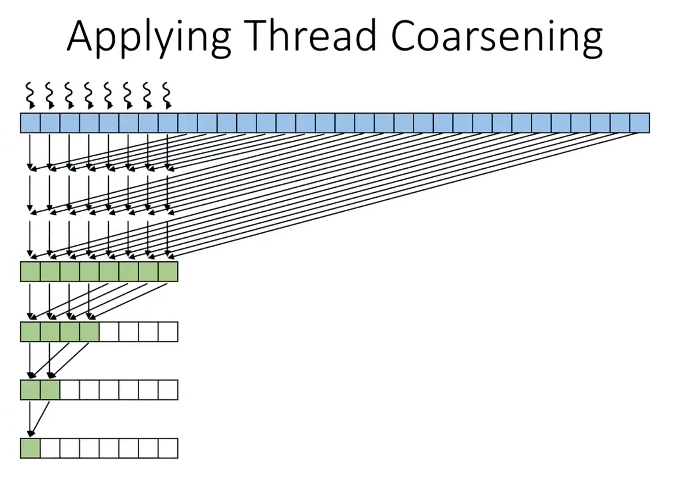
\includegraphics[width=0.8\textwidth]{images/reduction_coarsening.png}
\caption{thread coarsening}
\end{figure}
\begin{itemize}
\item Coarsening Benefits
\begin{itemize}
\item If blocks are all executed in parallel:
\begin{itemize}
\item $\log(N)$ steps, $\log(N)$ synchronizations
\end{itemize}
\item If blocks serialized by the hardware by a factor of C:
\begin{itemize}
\item $C*\log(N)$ steps, $C*\log(N)$ synchronizations
\end{itemize}
\item If blocks are coarsened by a factor of C:
\begin{itemize}
\item $2*(C - 1) + \log(N)$ steps, $\log(N)$ synchronizations

\end{itemize}
\end{itemize}
\end{itemize}

\newpage
\section{Scan (Kogge-Stone)}
scan


scan operation

\begin{itemize}
\item takes
\begin{itemize}
\item an input array $[x_0, x_1, \ldots, x_{n-1}]$
\item an associative operation $\oplus$, e.g. $+$, $\times$, $\max$, $\min$
\end{itemize}
\item returns
\begin{itemize}
\item an output array $[y_0, y_1, \ldots, y_{n-1}]$
\begin{itemize}
\item inclusive scan: $y_i = x_0 \oplus x_1 \oplus \ldots \oplus x_i$
\item exclusive scan: $y_i = x_0 \oplus x_1 \oplus \ldots \oplus x_{i-1}$

\end{itemize}
\end{itemize}
\end{itemize}
segmented scan (also called hierarchical scan)


\begin{figure}
\centering
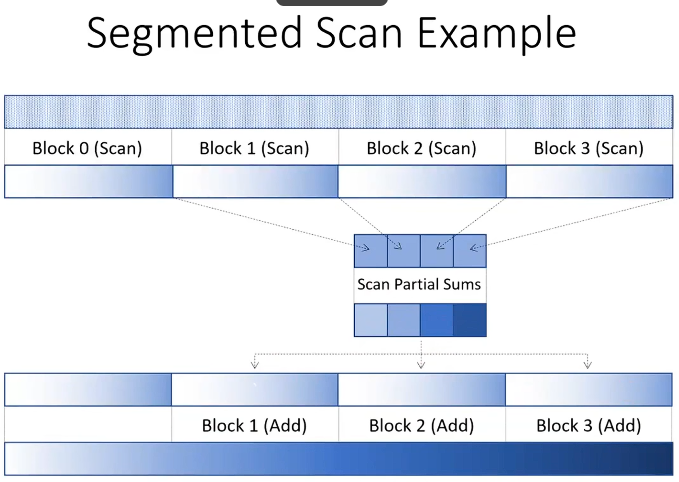
\includegraphics[width=0.8\textwidth]{images/image.png}
\caption{segmented scan}
\end{figure}

Kogge-Stone parallel (inclusive) scan


\begin{figure}
\centering
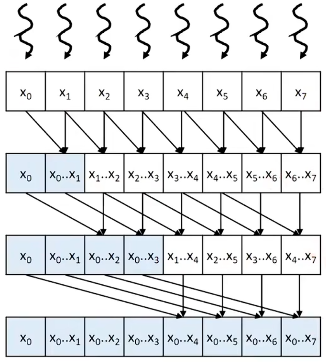
\includegraphics[width=0.8\textwidth]{images/image-1.png}
\caption{Kogge-Stone parallel (inclusive) scan}
\end{figure}

\begin{itemize}
\item careful with data races
\item \texttt{\_\_syncthreads()} in branch: undefined behavior
\item shared memory: buffer
\item double buffering: don't have to synchronize between read and write

\end{itemize}
exclusive scan: shift by one, insert identity element at the beginning


work efficiency

\begin{itemize}
\item A parallel algorithm is work efficient if it performs the same amount of work as the corresponding sequential algorithm

\end{itemize}
scan work efficiency

\begin{itemize}
\item sequential scan: $N$ additions
\item Kogge-Stone parallel scan
\begin{itemize}
\item $N-2^{step}$ operations per step, $\log N$ steps
\item total work: $N \log(N) - (N-1) = \mathcal{O}(N \log N)$ operations
\item not work efficient
\end{itemize}
\item Brent-Kung parallel scan
\begin{itemize}
\item Reduction: $\log(N)$ steps, $N-1$ operations
\item Post-reduction: $\log(N) - 1$ steps, $N-2 - (\log(N) - 1)$ operations
\item total: $2\log(N) - 1$ steps, $2N - \log(N) - 2 = \mathcal{O}(N)$ operations
\item takes more steps but more work efficient
\end{itemize}
\end{itemize}

\newpage
\section{Scan (Brent-Kung)}

Brent-Kung Parallel (Inclusive) Scan


\begin{figure}
\centering
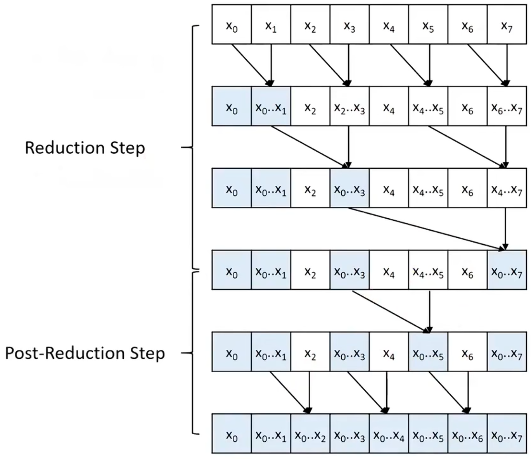
\includegraphics[width=0.8\textwidth]{images/image-2.png}
\caption{Brent-Kung Parallel (Inclusive) Scan}
\end{figure}

\begin{itemize}
\item using shared memory also enables coalescing (already coalesced in Kogge-Stone)
\item no need double-buffering
\item control divergence
\begin{itemize}
\item don't assign threads to specific data elements
\item re-index threads on every iteration to different elements
\begin{itemize}
\item reduction: using the right operand as the index
\item post-reduction: using the left operand as the index
\item when stride is $s$, thread $t$ is responsible for element $(t+1) \cdot (2s) - 1$

\end{itemize}
\end{itemize}
\end{itemize}
exclusive scan

\begin{itemize}
\item shift elements, or
\item different post-reduction step: Brent-Kung Parallel (Exclusive) Scan

\end{itemize}
\begin{figure}
\centering
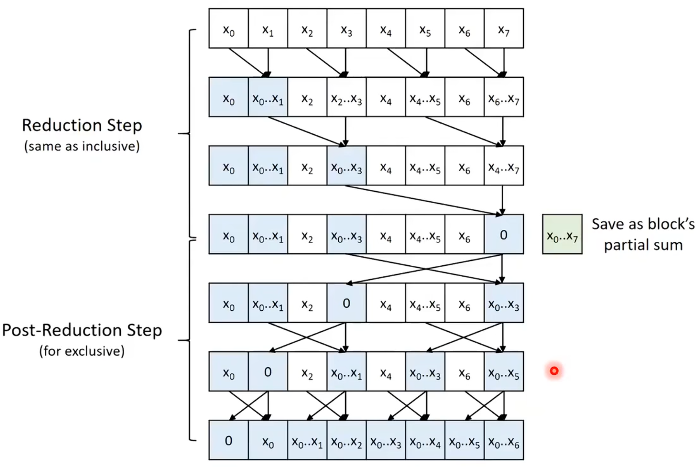
\includegraphics[width=0.8\textwidth]{images/image-3.png}
\caption{Brent-Kung Parallel (Exclusive) Scan}
\end{figure}

Thread Coarsening for scan

\begin{itemize}
\item each thread scans a segment sequentially
\item only scan the partial sums of each segment in parallel

\end{itemize}

\newpage
\section{Histogram}

Data races may result in unpredictable program output.


mutual exclusion

\begin{itemize}
\item CPU: locks (mutex)
\item atomic operation: read-modify-write with a single ISA instruction, serialized by the hardware

\end{itemize}
atomic operations in CUDA

\begin{itemize}
\item atomic add: \texttt{T atomicAdd(T* address, T val)}
\item function call translated to a single ISA instruction: instrinsics
\item sub, min, max, inc, dec, and, or, xor, exchange, compare and swap

\end{itemize}
atomic operations on global memory have high latency

\begin{itemize}
\item wait for both read and write to complete
\item wait if there are any other threads accessing the same location: high probablity of contension
\item optimize: privatization, coarsening, local counter

\end{itemize}
\textbf{privatization}: multiple private copies of an output are maintained, then the global copy is updated on completion

\begin{itemize}
\item operations on the output must be associative and commutative

\end{itemize}

\newpage
\section{Merge}

ordered merge


parallelization

\begin{itemize}
\item each thread for a segment of output array
\item finding input segments, binary search co-rank $i$ ($j=k-i$)
\begin{itemize}
\item bound on $i$: $\max(0,k-n)\leq i \leq \min(k,m)$
\item guess is correct: $A[i-1]\leq B[j]$ and $B[j-1]\leq A[i]$
\item guess is too high: $A[i'-1]>B[j']$
\item guess is too low: $B[j''-1]>A[i'']$

\end{itemize}
\end{itemize}
\begin{figure}
\centering
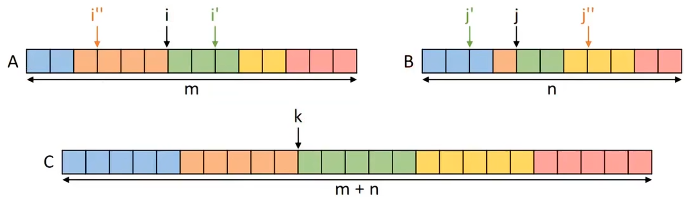
\includegraphics[width=0.8\textwidth]{images/image-8.png}
\caption{Finding Input Segments}
\end{figure}

memory accesses are not coalesced, optimization

\begin{itemize}
\item load the block's segment to shared memory
\item do the per-thread co-rank and merge in shared memory
\item already applied thread coarsening

\end{itemize}
\begin{figure}
\centering
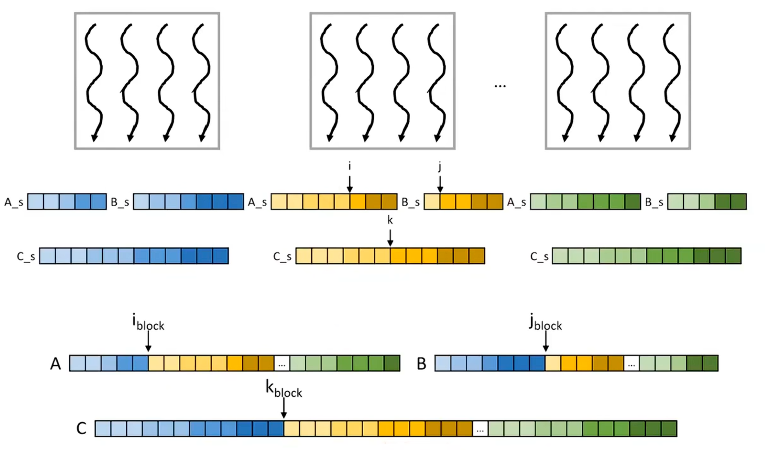
\includegraphics[width=0.8\textwidth]{images/image-9.png}
\caption{Shared Memory Tiling}
\end{figure}

\newpage
\section{Sort}

radix sort

\begin{itemize}
\item distribute keys into buckets based on a radix (or base)
\item distributing keys into buckets is repeated for each digit, while preserving the order from previous iterations
\item using a radix that is a power of 2 simplifies processing binary numbers
\begin{itemize}
\item each iteration handles a fixed slice of bits from the keys
\end{itemize}
\item is not a comparison-based sort, so it's not applicable to all kinds of keys

\item finding destination index
\begin{itemize}
\item need to find: \#ones to the left of each element
\begin{itemize}
\item destination of a zero = element index - \#ones to the left
\item destination of a one = input size - \#ones in total + \#ones to the left
\item use exclusive scan
\end{itemize}
\item extract bit -> exclusive scan -> destination index -> take and store

\end{itemize}
\end{itemize}
\begin{figure}
\centering
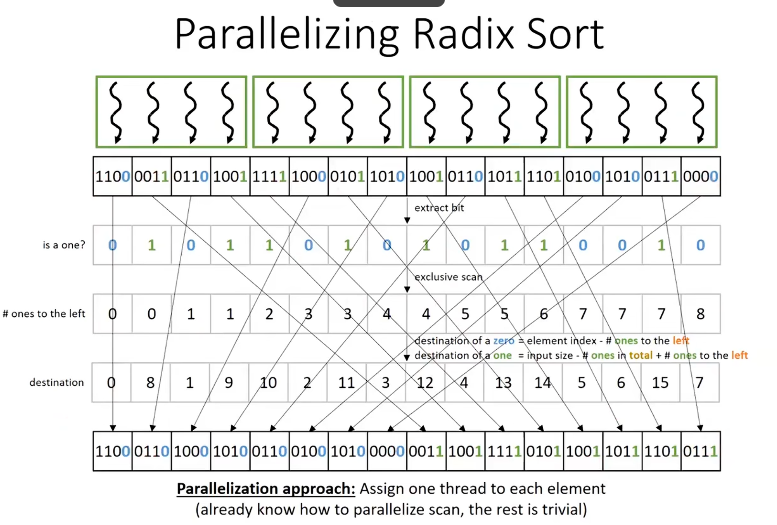
\includegraphics[width=0.8\textwidth]{images/image-4.png}
\caption{paralleling radix sort}
\end{figure}

stores are not coalesced

\begin{itemize}
\item sort locally in shared memory, then write each bucket to global memory in a coalesced manner

\end{itemize}
\begin{figure}
\centering
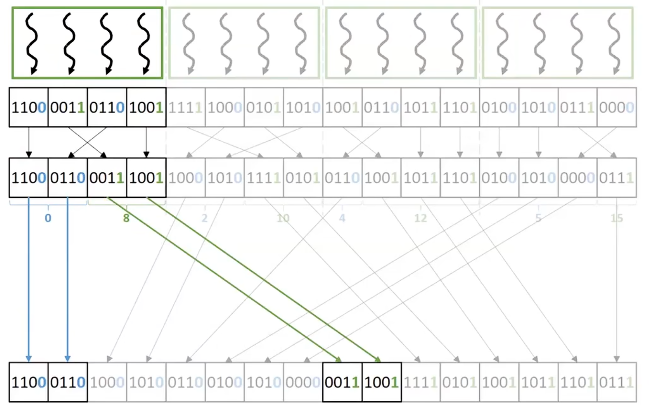
\includegraphics[width=0.8\textwidth]{images/image-5.png}
\caption{optimizing memory coalescing}
\end{figure}

choice of radix value

\begin{itemize}
\item larger radix
\begin{itemize}
\item advantage: fewer iterations
\item disadvantage: more buckets, results in poorer coalescing

\end{itemize}
\end{itemize}
thread coarsening  


\begin{figure}
\centering
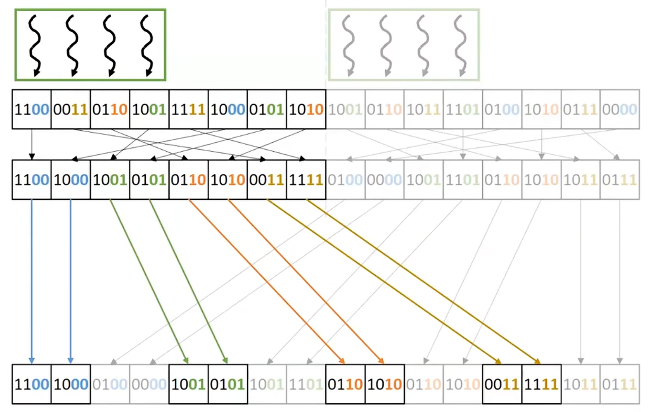
\includegraphics[width=0.8\textwidth]{images/image-6.png}
\caption{Radix Sort with Thread Coarsening}
\end{figure}

merge sort

\begin{itemize}
\item divide the list into sublists, sorts the sublists, then merges them (divide and conquer algorithm)

\end{itemize}
\begin{figure}
\centering
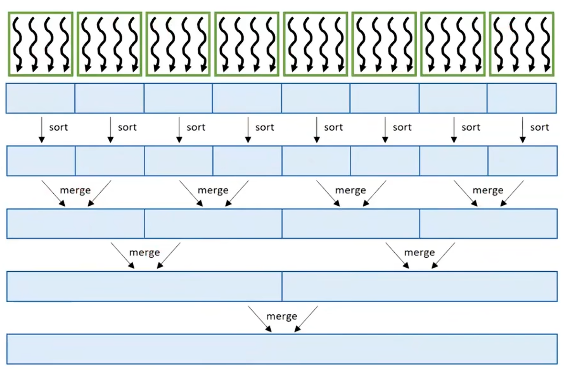
\includegraphics[width=0.8\textwidth]{images/image-7.png}
\caption{Merge Sort}
\end{figure}
\begin{itemize}
\item early steps rely more on parallelism across merge operations
\item later steps rely more on parallelism within merge operations
\end{itemize}

\newpage
\section{Sparse Matrix (COO, CSR)}

sparse matrices: many elements are zero


opportunities

\begin{itemize}
\item do not need to allocate space for zeros (save memory)
\item do not need to load zeros (save memory bandwidth)
\item do not need to compute with zeros (save computation time)

\end{itemize}
sparse matrix storage formats

\begin{itemize}
\item Coordinate Format (COO)
\item Compressed Sparse Row (CSR)
\item ELLPACK Format (ELL)
\item Jagged Diagonal Storage (JDS)
\item ...

\end{itemize}
format design considerations

\begin{itemize}
\item space efficiency (memory consumed)
\item flexibility (ease of adding/reordering elements)
\item accessibility (ease of finding desired data)
\item memory access patterns (enabling coalescing)
\item load balance (minimizing control divergence)

\end{itemize}
case study: sparse matrix-vector multiplication (SpMV)

\begin{itemize}
\item the produnct of a sparse matrix and a dense vector

\end{itemize}
Coordinate Format (COO)

\begin{itemize}
\item stores every nonzero along with its row index and column index

\end{itemize}
SpMV/COO

\begin{itemize}
\item assign one thread per nonzero
\item multiple threads writing to the same output, need atomic operations
\item already coalesced

\end{itemize}
\begin{figure}
\centering
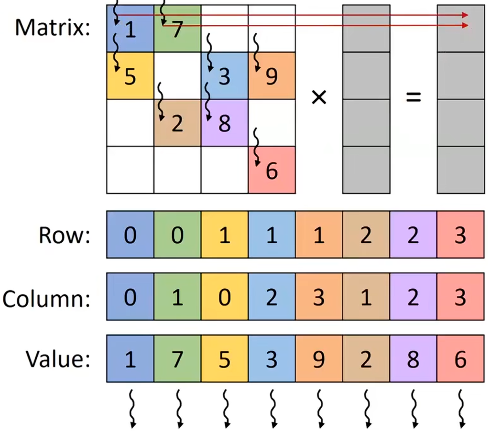
\includegraphics[width=0.8\textwidth]{images/image-11.png}
\caption{SpMV/COO}
\end{figure}

COO tradeoffs

\begin{itemize}
\item advantages
\begin{itemize}
\item flexiblity: easy to add new elements, nonzeros can be stored in any order
\item accessibility: given a nonzero, can easily find its row and column
\item SpMV/COO has coalesced memory access and no control divergence
\end{itemize}
\item disadvantages
\begin{itemize}
\item accessibility: given a row and column, hard to find all nonzeros
\item SpMV/COO requires atomic operations

\end{itemize}
\end{itemize}
Compressed Sparse Row (CSR)

\begin{itemize}
\item stores nonzeros of the same row adjacently and an index to the first element of each row

\end{itemize}
SpMV/CSR

\begin{itemize}
\item assign one thread per row

\end{itemize}
\begin{figure}
\centering
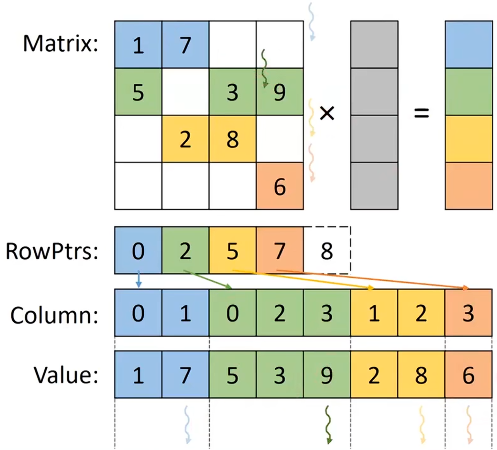
\includegraphics[width=0.8\textwidth]{images/image-10.png}
\caption{SpMV/CSR}
\end{figure}

CSR tradeoffs

\begin{itemize}
\item advantages
\begin{itemize}
\item space efficiency: row pointers smaller than column indices
\item accessibility: given a row, easy to find all nonzeros
\item SpMV/CSR avoids atomics
\end{itemize}
\item disadvantages
\begin{itemize}
\item flexibility: hard to add new elements
\item accessibility: given nonzero, hard to find its row; given a column, hard to find all nonzeros
\item SpMV/CSR has uncoalesced memory access and control divergence

\end{itemize}
\end{itemize}
Compressed Sparse Column (CSC): like CSR but groups nonzeros by column


\newpage
\section{Sparse Matrix (ELL, JDS)}

ELLPACK Format (ELL)

\begin{itemize}
\item pad each row to the same size
\item store padded array in column-major order

\end{itemize}
SpMV/ELL

\begin{itemize}
\item assign one thread to loop over each input row sequentially

\end{itemize}
\begin{figure}
\centering
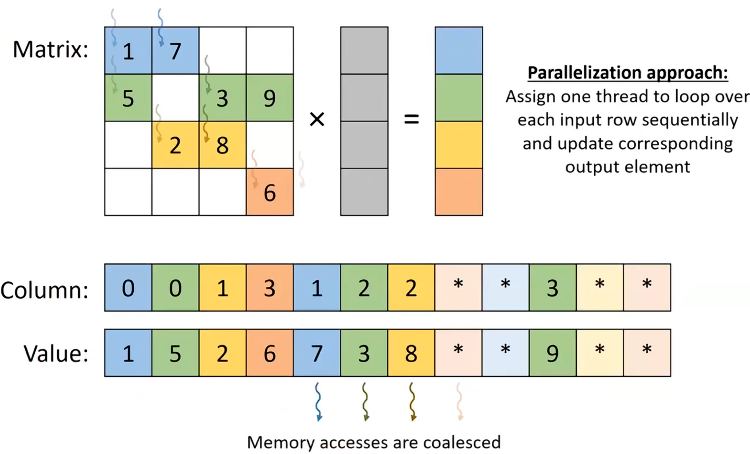
\includegraphics[width=0.8\textwidth]{images/image-12.png}
\caption{SpMV ELL}
\end{figure}

ELL tradeoffs

\begin{itemize}
\item advantages
\begin{itemize}
\item flexibility: can add new elements as long as row not full
\item accessibility: given row, easy to find all nonzeros; given non-zero, easy to find its row and column
\item SpMV/ELL memory access is coalesced
\end{itemize}
\item disadvantages
\begin{itemize}
\item space efficiency: overhead due to padding
\item accessibility: given column, hard to find all nonzeros
\item SpMV/ELL has control divergence

\end{itemize}
\end{itemize}
Hybrid ELL + COO: use COO for very long rows


\begin{figure}
\centering
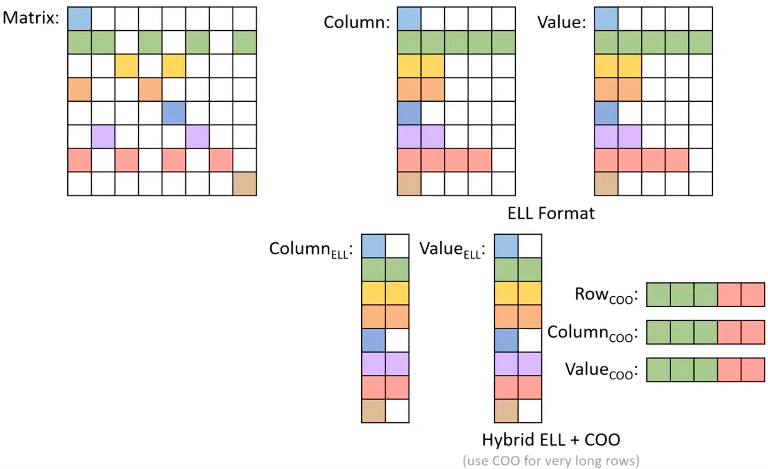
\includegraphics[width=0.8\textwidth]{images/image-13.png}
\caption{Hybrid ELL COO}
\end{figure}

\begin{itemize}
\item benefits
\begin{itemize}
\item space efficient: less padding
\item flexibility: can add new elements to any row
\end{itemize}
\item still has control divergence

\end{itemize}
Jagged Diagonal Storage (JDS)

\begin{itemize}
\item sort rows by size and remember the original row index
\item store nonzeros in column major
\item remember where the nonzeros of each iteration start (\texttt{IterPtr})

\end{itemize}
SpMV/JDS

\begin{itemize}
\item assign one thread to loop over each input row sequentially and update corresponding output element

\end{itemize}
\begin{figure}
\centering
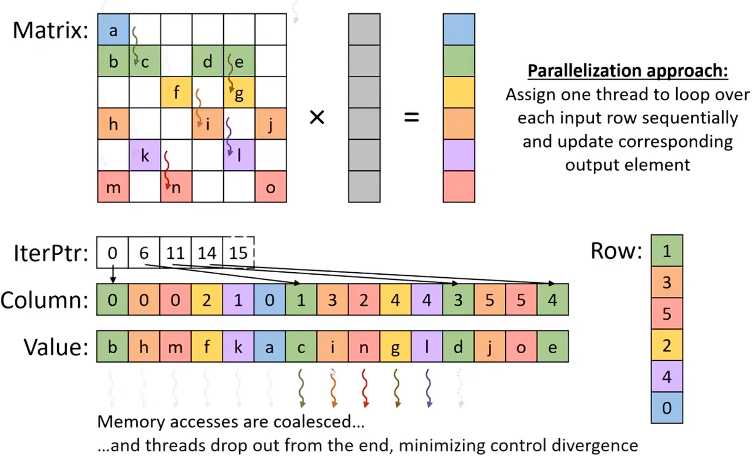
\includegraphics[width=0.8\textwidth]{images/image-14.png}
\caption{SpMV JDS Kernel}
\end{figure}

JDS tradeoffs

\begin{itemize}
\item advantages
\begin{itemize}
\item space efficient: no padding
\item accessibility: given a row, easy to find all nonzeros
\item SpMV/JDS memory access is coalesced
\item SpMV/JDS minimizes control divergence
\end{itemize}
\item disadvantages
\begin{itemize}
\item flexibility: hard to add new elements to the matrix
\item accessibility: given nonzero, hard to find row; given a column, hard to find all nonzeros
\end{itemize}
\end{itemize}

\newpage
\section{Graph Algorithms I}

representing graphs: adjacency matrices


focus on

\begin{itemize}
\item unweighted graph: 1 for edge, 0 for no edge
\item undirected graph: symmetric adjacency matrix

\end{itemize}
COO and CSR/CSC representations

\begin{itemize}
\item COO: array \texttt{src}, array \texttt{dst}
\item CSR and CSC are equivalent because of symmetry: array \texttt{srcPtrs}, array \texttt{dst}

\end{itemize}
parallelizing graph processing

\begin{itemize}
\item vertex-centric
\begin{itemize}
\item assign a thread to do something for each vertex
\item typically use CSR/CSC (might ELL, JDS, ...) : given a vertex, easy to find its neighbors
\end{itemize}
\item edge-centric
\begin{itemize}
\item assign a thread to do something for each edge
\item typically use COO: given an edge, easy to find its source and destination
\end{itemize}
\item hybrid
\begin{itemize}
\item example: given an edge, need neighbors of its source and destination, need both COO and CSR/CSC
\begin{itemize}
\item triangle counting, k-core decomposition, ...

\end{itemize}
\end{itemize}
\end{itemize}
Breadth First Search (BFS) 

\begin{itemize}
\item vertex-centric (2 versions)
\begin{itemize}
\item top-down: for every vertex in the previous level, add all its unvisited neighbors to the current level
\begin{itemize}
\item i.e. assign a thread to every parent vertex in the BFS tree
\end{itemize}
\item bottom-up: for every vertex, if it has not been visited, if any of its neighbors is in the previous level, add it to the current level
\begin{itemize}
\item i.e. assign a thread to every potential child vertex in the BFS tree
\end{itemize}
\item direction-optimized: start with top-down then switch to bottom-up
\end{itemize}
\item edge-centric
\begin{itemize}
\item for every edge, if its source was in the previous level, add its destination to the current level

\end{itemize}
\end{itemize}
\begin{figure}
\centering
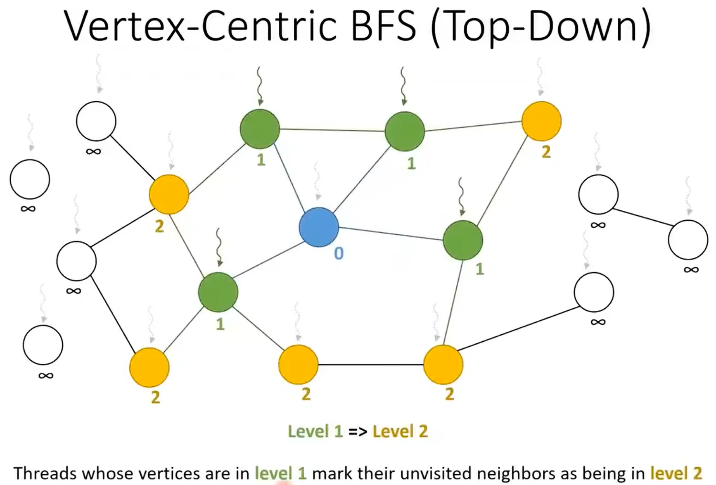
\includegraphics[width=0.8\textwidth]{images/image-16.png}
\caption{Vertex-Centric BFS (Top-Down)}
\end{figure}
\begin{figure}
\centering
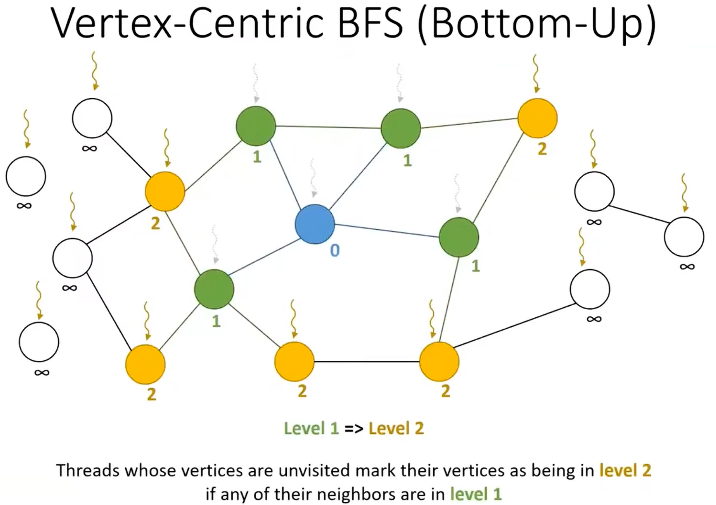
\includegraphics[width=0.8\textwidth]{images/image-15.png}
\caption{Vertex-Centric BFS (Bottom-Up)}
\end{figure}
\begin{figure}
\centering
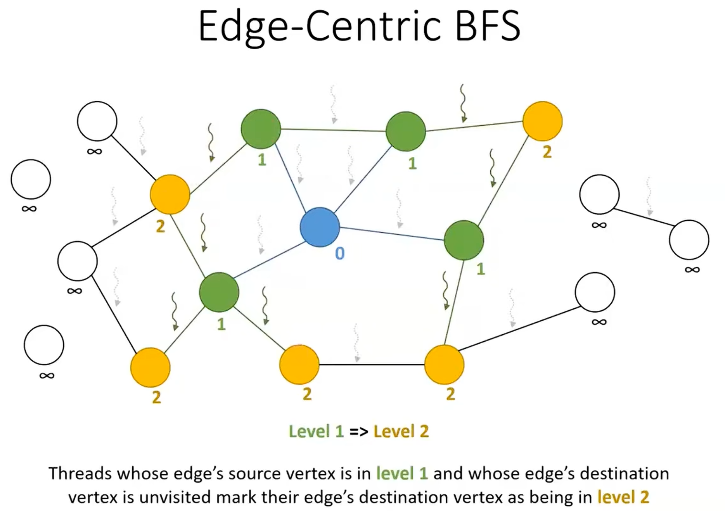
\includegraphics[width=0.8\textwidth]{images/image-17.png}
\caption{Edge-Centric BFS}
\end{figure}

Notice: there should be 2 threads per edge in the image because the graph is undirected, but only show one for simplicity.


Dataset Implications

\begin{itemize}
\item the best parallelization approach depends on the structure of the graph
\item the vertex-centric bottom-up and edge-centric approaches are better on high-degree graphs
\begin{itemize}
\item e.g. social network graphs with celebrities
\item better at dealing with load imbalance
\end{itemize}
\item the vertex-centric top-down approach is better on low-degree graphs
\begin{itemize}
\item e.g. map of roads in a geographical area
\item can be improved by launching more threads to process neighbors of high-degree vertices

\end{itemize}
\end{itemize}
\begin{figure}
\centering
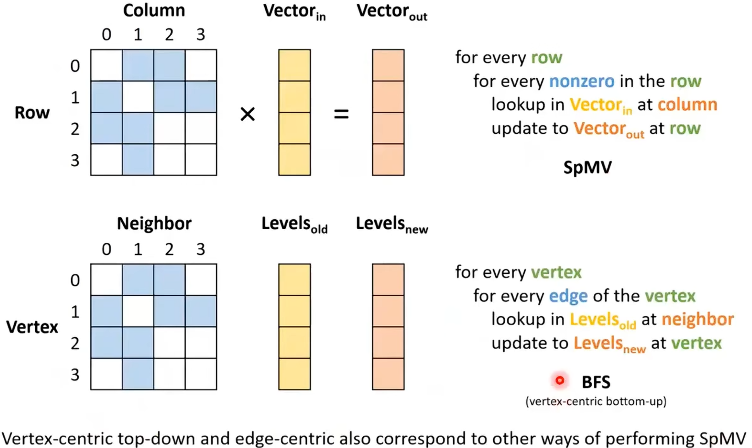
\includegraphics[width=0.8\textwidth]{images/image-18.png}
\caption{Similarity between BFS and SpMV}
\end{figure}

Linear Algebraic Formulation of Graph Problems

\begin{itemize}
\item with a few tweaks, BFS can be formulated as SpMV
\begin{itemize}
\item use visited list as input/output vector
\item a few other operations to get wanted
\end{itemize}
\item Many graph problems can be formulated in terms of sparse linear algebra computations
\begin{itemize}
\item advantage: leverage mature and well-optimized parallel libraries for high performance sparse linear algebra
\item disadvantage: not always the most efficient way to solve the problem

\end{itemize}
\end{itemize}
Redundant Work

\begin{itemize}
\item approaches so far check every vertex/edge on every iteration for relevance
\item easy to implement, highly parallel, no synchronization across threads
\item weakness: a lot of unnecessary threads/work
\begin{itemize}
\item many threads will find that their vertex/edge is not relevant for this iteration and just exit

\end{itemize}
\end{itemize}

\newpage
\section{Graph Algorithms II}

Remark: if not symmetric, top-down BFS need CSR representation, while bottom-up BFS need CSC representation, (treating rows as source) dir-opt BFS need both CSR and CSC.


Reduce Redundancy

\begin{itemize}
\item objective: only check the vertices that are part of the previous level
\item approach: each level places the vertices it visits in a queue for the next level to process
\begin{itemize}
\item vertices enqueued at each level form that level's frontier
\end{itemize}
\item overhead: synchronization across threads to add to a shared queue

\end{itemize}
\begin{figure}
\centering
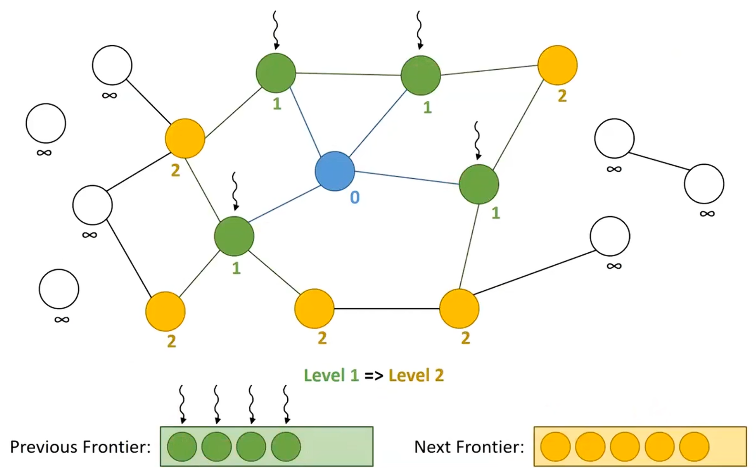
\includegraphics[width=0.8\textwidth]{images/image-19.png}
\caption{Vertex-Centric Frontier-Based BFS}
\end{figure}

Queue Privatization

\begin{itemize}
\item all threads atomically increment the same global counter to insert elements into the queue, high latency due to global memory access and serialization due to high contention.
\item optimization: each thread block maintains a private queue (in shared memory, with the counter) and commits entries to the global queue on completion

\end{itemize}
Minimizing Launch Overhead

\begin{itemize}
\item need to synchronize between levels
\item so far, we have launched a new grid for each level
\begin{itemize}
\item overhead of launching new grid and copying counter
\end{itemize}
\item optimization: if consecutive levels have few enough vertices that can be executed by one thread block:
\begin{itemize}
\item execute multiple levels in one single-block grid and synchronize between levels using \_\_syncthreads()
\item reduce total number of grid launches

\end{itemize}
\end{itemize}
\begin{figure}
\centering
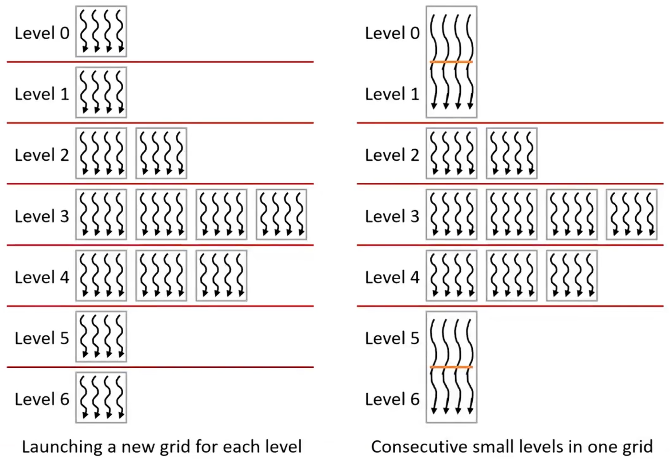
\includegraphics[width=0.8\textwidth]{images/image-20.png}
\caption{Minimizing Launch Overhead}
\end{figure}



\newpage
\section{Warp Synchronization}

\subsection{intra-warp synchronization}

take advantage of the special relationship between threads in the same warp to synchronize quickly


CUDA has several built-in functions to synchronize between warps

\begin{itemize}
\item sharing (shuffling) data across threads
\item voting across threads

\end{itemize}
\subsection{shuffle}

built-in warp shuffle functions enable threads to share data with other threads in the same warp

\begin{itemize}
\item faster than shared memory and \texttt{\_\_syncthreads()} cross the block
\end{itemize}
\begin{itemize}
\item variants
\begin{itemize}
\item \texttt{\_\_shfl\_sync()}: direct copy from indexed lane
\item \texttt{\_\_shfl\_up\_sync()}: copy from a lane with lower ID relative to the caller
\item \texttt{\_\_shfl\_down\_sync()}: copy from a lane with higher ID relative to the caller
\item \texttt{\_\_shfl\_xor\_sync()}: copy from a lane based on a bitwise XOR of own lane ID

\end{itemize}
\end{itemize}
example: reduction/scan

\begin{itemize}
\item When one warp remains, use \texttt{\_\_shfl\_down\_sync()} to share data from registers

\end{itemize}
\subsection{voting}

built-in warp vote functions enable threads to vote on which threads in the warp satisfy some condition

\begin{itemize}
\item \texttt{\_\_all\_sync(unsigned mask, predicate)}: check if predicate is nonzero for all threads
\item \texttt{\_\_any\_sync(unsigned mask, predicate)}: check if predicate is nonzero for any thread
\item \texttt{\_\_ballot\_sync(unsigned mask, predicate)}: return mask of which threads evaluate predicate to nonzero
\item \texttt{\_\_activemask()}: return mask of which threads are active

\end{itemize}
example: enqueue, have only one thread in the warp increment the counter on behalf of the others

\begin{enumerate}
\item assign a leader thread
\begin{itemize}
\item find the active threads in the warp using \texttt{\_\_activemask()}
\item disignate the first active thread as the leader using \texttt{\_\_ffs(mask) - 1}
\begin{itemize}
\item index of \texttt{\_\_ffs(mask)} starts from 1, returns 0 if no bits are set
\end{itemize}
\end{itemize}
\item find how many threads need to enqueue
\begin{itemize}
\item use \texttt{\_\_popc(mask)} to count the number of set bits in the mask
\end{itemize}
\item have the leader perform the atomic operation
\begin{itemize}
\item threads in the same warp are consecutive, so \texttt{threadIdx.x \% WARP\_SIZE} gives the position in the warp
\end{itemize}
\item broadcast the result to the other threads
\begin{itemize}
\item use \texttt{\_\_shfl\_sync(mask, j, leader)}
\end{itemize}
\item find offset of each active thread and store the result
\begin{itemize}
\item use bitwise AND to find the number of previous active threads

\end{itemize}
\end{enumerate}
Gemini's suggestions:

\begin{enumerate}
\item Replaced \texttt{\_\_activemask()} with \texttt{\_\_ballot\_sync(0xffffffff, is\_active)}: On modern GPU architectures (Volta and above), independent thread scheduling can cause \texttt{\_\_activemask()} to return only a subset of active threads taking a divergent branch. Using \texttt{\_\_ballot\_sync} guarantees all evaluating threads in the warp are grouped together, preventing multiple partial \texttt{atomicAdd}s.
\item Changed \texttt{1 << ...} to \texttt{1u << ...}: This avoids undefined behavior from signed integer overflow when the thread index is 31.
\end{enumerate}

\newpage
\section{Pinned Memory and Streams}

\subsection{Pinned Memory}

Direct Memory Access (DMA) allows some hardware to access memory without involving the CPU

\begin{itemize}
\item copying between CPU and GPU uses DMA
\item advantage: CPU can be utilized for other tasks while the memory copy is taking place
\item DMA use physical addresses to access memory, cannot detect if the OS swaps a virtual page with another virtual page at the same physical address
\item to avoid data corruption, the OS must not be allowed to swap pages being accessed by DMA
\item pages to be accessed by DMA must be allocated as pinned memory (also called page-locked memory), marked as non-swappable by the OS

\end{itemize}
cudaMemcpy

\begin{itemize}
\item host to device: CPU copies data to a pinned memory buffer, DMA copies data from pinned memory buffer to the device
\item device to host: DMA copies data from the device to a pinned memory buffer, CPU copies data from pinned memory buffer
\item disadvantage: every cudaMemcpy is actually two copies, which incurs overhead

\end{itemize}
faster copies: allocate host arrays directly in pinned memory

\begin{itemize}
\item \texttt{cudaError\_t cudaMallocHost(void **devPtr, size\_t size)}
\item \texttt{cudaError\_t cudaFreeHost(void *devPtr)}
\item use with caution: only use for frequently copied data if overhead is high
\item allocating too much pinned memory degrades overall system performance by reducing the virtual pages available for swapping

\end{itemize}
\subsection{Stream}

Typical system is simultaneously capable of

\begin{itemize}
\item executing grids on the GPU
\item copying from host to device
\item copying from device to host

\end{itemize}
Example: previous timeline of vector addition

\begin{itemize}
\item copy A to device
\item copy B to device
\begin{itemize}
\item not utilizing GPU and copyDeviceToHost
\end{itemize}
\item execute grid to compute A+B
\begin{itemize}
\item not utilizing copies
\end{itemize}
\item copy C from device
\begin{itemize}
\item not utilizing GPU and copyHostToDevice

\end{itemize}
\end{itemize}
pipelining vector addition

\begin{itemize}
\item divide arrays into segments
\item overlap copy and computation of different segments

\end{itemize}
\begin{figure}
\centering
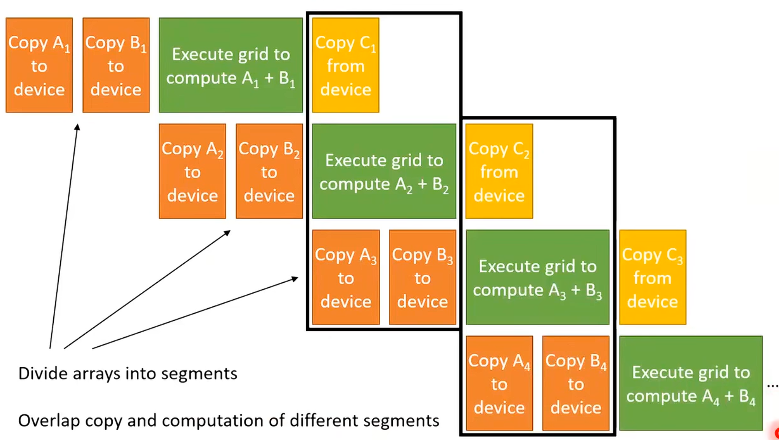
\includegraphics[width=0.8\textwidth]{images/image-21.png}
\caption{Pipelining Vector Addition}
\end{figure}

streams and asynchronous copies

\begin{itemize}
\item parallelism between grids and memory copies is achieved by using \textbf{streams}
\begin{itemize}
\item tasks in different streams are executed in parallel
\item tasks in the same stream are serialized
\item if no stream is specified, tasks go into the default stream
\end{itemize}
\item to overlap memory copies with host execution, use \textbf{asynchronous memory copies}
\item \texttt{cudaError\_t cudaStreamCreate(cudaStream\_t *pStream)}
\item \texttt{cudaError\_t cudaMemcpyAsync(void *dst, const void *src, size\_t count, cudaMemcpyKind kind, cudaStream\_t stream=0)}
\item \texttt{kernel<<<blocks, threads, smem, stream>>>(...)}
\item cudaEvent\_t can be used to measure the time taken in different streams


\end{itemize}

\newpage
\section{Dynamic Parallelism}

Dynamic Parallism: CUDA dynamic parallelism refers to the ability of threads executing on the GPU to launch new grids


Nested Parallelism: Dynamic parallelism is useful for programming applications with nested parallelism, where each thread discovers more work that can be parallelized; particularly useful when the amount of nested work is unknown, so enough threads cannot be launched up front.


applications

\begin{itemize}
\item nested parallel work is \textbf{irregular} (varies cross threads)
\begin{itemize}
\item e.g. graph algorithms (eacb vertex has a different number of neighbors)
\item e.g. Bezier curve (each curve needs different number of points to draw)
\end{itemize}
\item nested parallel work is \textbf{recursive} with unknown depth
\begin{itemize}
\item e.g. tree traversal algorithms (e.g., quadtrees and octrees)
\item e.g. divide and conquer algorithms (e.g., quicksort)

\end{itemize}
\end{itemize}
\begin{figure}
\centering
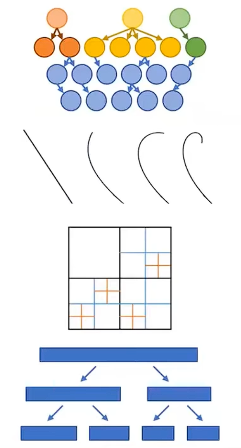
\includegraphics[width=0.8\textwidth]{images/image-22.png}
\caption{Applications of Dynamic Parallism}
\end{figure}

\begin{itemize}
\item the device code for calling a kernel to launch a grid is the same as the host code
\item memory is needed for buffering grid launches that have not started executing
\begin{itemize}
\item The limit on the number of dynamic launches is referred to as the \textbf{pending launch count}
\item By default, the runtime supports 2048 launches, and exceeding this limit will cause an error
\item The limit can be increased by setting \texttt{cudaDeviceSetLimit(cudaLimitDevRuntimePendingLaunchCount, <new limit>)}

\end{itemize}
\end{itemize}
example: graph frontier BFS

\begin{itemize}
\item Directly launching child\_kernel behaves worse
\end{itemize}
\begin{enumerate}
\item for device launches, threads in the same block share the same default stream (serialized)
\end{enumerate}
\begin{itemize}
\item improve by creating a different stream per thread
\begin{itemize}
\item use \texttt{cudaStreamCreate} as host, or
\item use compiler flag \texttt{--default-stream per-thread}
\end{itemize}
\end{itemize}
\begin{enumerate}
\item Pitfalls
\begin{itemize}
\item launching very small grids may not be worth the overhead (more efficient to serialize)
\item launching too many grids causes queuing delays
\end{itemize}
\item Optimization: apply a threshold to the launch
\begin{itemize}
\item only launch the large grids that are worth the overhead, and serialize the rest
\item threshold value is data dependent and can be tuned
\end{itemize}
\item Optimization: aggregate launched
\begin{itemize}
\item have one thread collect the work of multiple threads and launch a single grid on their behalf

\end{itemize}
\end{enumerate}
Offloading Driver Code

\begin{itemize}
\item free up the host to do other things
\item notice: for single thread, CPU code is faster than GPU code, so it's unworthy in many cases

\end{itemize}
Memory Visibility

\begin{itemize}
\item Operations on global memory made by a parent thread before the launch are visible to the child threads
\item Operations made by the child are visible to the parent after the child returns and the parent has synchronized
\item A thread's local memory and a block's shared memory cannot be accessed by child threads

\end{itemize}
Nesting Depth: how deeply dynamically launched grids may launch other grids

\begin{itemize}
\item determined by the hardware (typically 24)





\end{itemize}

\newpage
\section{CUDA Potpourri}

\subsection{Multi-GPU programming}

multiple GPUs on the same node

\begin{itemize}
\item \texttt{cudaGetDeviceCount}
\item \texttt{cudaSetDevice} to select one
\item typically use multiple CPU threads with one driving each GPU (e.g. using OpenMP)

\end{itemize}
multiple GPUs on multiple different nodes

\begin{itemize}
\item typically use MPI for programming multiple nodes, and each MPI rank interacts with its GPU normally
\item important consideration: overlapping MPI communication with kernel execution

\end{itemize}
\subsection{Interconnect}

\begin{itemize}
\item PCIe: general, widely supported
\item NVLink: faster between multi-GPUs, but only supported on some GPUs and some CPUs

\end{itemize}
\subsection{Memory management}

Unified Virtual Addressing (UVA)

\begin{itemize}
\item $\text{CPU} \longleftrightarrow \substack{\boxed{\text{Main Memory} \longleftrightarrow \text{Global Memory}}\\\text{UVA space}} \longleftrightarrow \text{GPU}$
\item advantage: data location is known from the pointer value, so do not need to specify copy direction
\begin{itemize}
\item \texttt{cudaMemcpyDefault}
\end{itemize}
\item simpler code
\item performance depends on situation

\end{itemize}
Zero-copy memory: enables devices to directly access host memory

\begin{itemize}
\item memory has to be pinned
\item \texttt{cudaHostAlloc(\&ptr, size, cudaHostAllocMapped)} to allocate the memory
\item \texttt{cudaHostGetDevicePointer} to get corresponding device pointer
\begin{itemize}
\item unnecessary if using UVA

\end{itemize}
\end{itemize}
\subsection{Events}

\begin{itemize}
\item synchronizing after every copy or kernel call interferes with execution and slows things down
\item Events can be used to collect timing information without synchronizing
\begin{itemize}
\item \texttt{cudaEventCreate(\&event)}
\item \texttt{cudaEventRecord(event, stream=0)}
\item \texttt{cudaEventSynchronize(event)}
\item \texttt{cudaEventElapsedTime(\&result, startEvent, endEvent)}
\item \texttt{cudaEventDestroy(event)}
\end{itemize}
\item profilers can also be used

\end{itemize}
\subsection{Tensor cores}

programmable matrix multiplication and accumulation units

\begin{itemize}
\item accelerate DNN workloads
\item in Volta v100, 640 cores (8 per SM), each core is capable of a 4x4 matrix multiply-accumulate operation D = A * B + C

\end{itemize}
\subsection{Libraries}

examples of libraries for common parallel primitives

\begin{itemize}
\item Thrust: reduction, scan, filter, and sort
\item cuBLAS: basic dense linear algebra
\begin{itemize}
\item NVBLAS: multi-GPU library on top of cuBLAS
\end{itemize}
\item cuSPARSE: sparse-dense linear algebra
\item cuSOLVER: factorization and solve routines, on top of cuBLAS and cuSPARSE
\item cuDNN: deep neural networks
\begin{itemize}
\item used by Caffe, TensorFlow, PyTorch, MxNet, etc.
\end{itemize}
\item nvGRAPH: graph processing
\item cuFFT: Fast Fourier Transform
\item NPP: signal, image, and video processing

\end{itemize}
\subsection{Other programming interfaces}

\begin{itemize}
\item OpenCL: similar to CUDA, but open source and more portable across non-NVIDIA GPUs
\item OpenACC: directive-based GPU programming
\begin{itemize}
\item annotate code similar to OpenMP
\end{itemize}
\item C++AMP: implementing GPU programs directly in C++

\end{itemize}
\subsection{Other hardware}

other GPUs

\begin{itemize}
\item AMD (Radeon)
\item ARM (Mali)
\item Intel

\end{itemize}
integrated GPUs


FPGA


\subsection{Comparison with CPU}

more fair to compare with parallel and vectorized CPU code


\newpage
\section{Matrix Multiplication Optimization}

the simple matrix multiplication kernel is memory bound

\begin{itemize}
\item arithmetic intensity is 0.25 FLOP/B
\item higher in practice due to caches, but still memory bound
\end{itemize}
but matrix multiplication has the potential to be highly compute bound (so it suits GPU well)

\begin{itemize}
\item for $N$-$N$ square matrices, data accessed is $12N^2$ B, operations is $2N^3$ FLOP, so arithmetic intensity is $N/6$ FLOP/B
\item h100 approximately 20 FLOP/B

\end{itemize}
review: tiled matrix-matrix multiplication

\begin{itemize}
\item input in shared memory, output in registers
\item for $n$-$n$ square tiles (ignore storage), ($2n^3$ FLOP) / ($8n^2$ B) = $0.25n$ FLOP/B, $8$ FLOP/B for $n=32$
\item increasing $n$

\end{itemize}
Let the tiles of A, B, C have size $m\cdot k$, $k\cdot n$, $m\cdot n$

\begin{itemize}
\item arithmetic intensity: $(mn)(k\text{ adds}+k\text{ muls})/((mk+kn\text{ values})(4\text{ B})) = 0.5mn / (m+n)$ FLOP/B
\item increasing $m$ and $n$ increases reuse ratio, keeping $k$ small prevents increasing demand on shared memory, but stress on registers
\item typically use $m=n=128$, $k=8$, achieving 32 FLOP/B, $k$ not too small to utilize caches
\begin{itemize}
\item use 256 threads per block, 8x8 elements per thread

\end{itemize}
\end{itemize}
By default, local memory arrays are placed in the global memory

\begin{itemize}
\item with loop unrolling, variable indices are converted to constant indices which allows the compiler to promote the arrays to registers
\item e.g. \texttt{\_\_forceinline\_\_} with \texttt{\#pragma unroll}

\end{itemize}
\begin{figure}
\centering
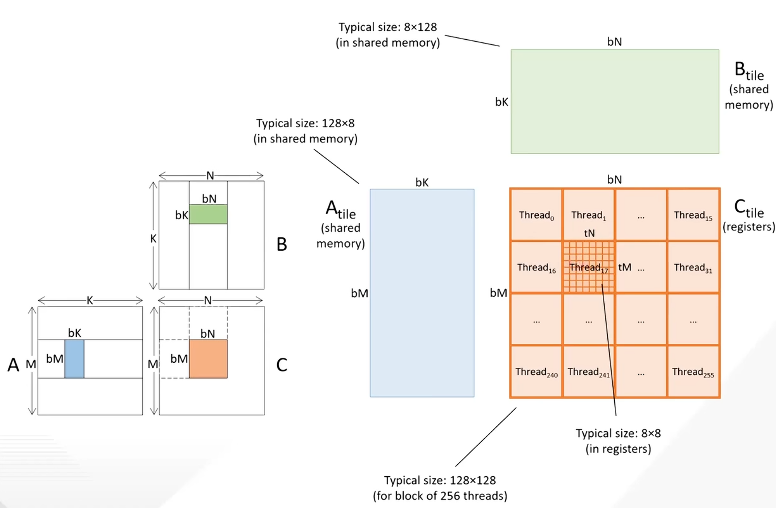
\includegraphics[width=0.8\textwidth]{images/image-24.png}
\caption{Use Large Tiles}
\end{figure}
\begin{figure}
\centering
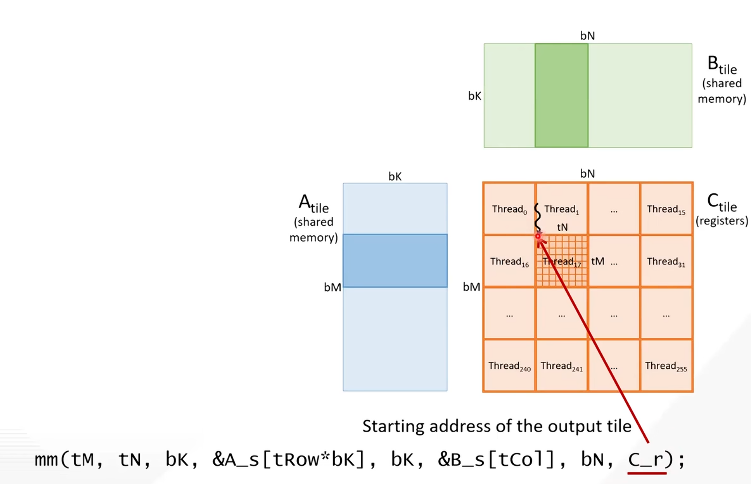
\includegraphics[width=0.8\textwidth]{images/image-23.png}
\caption{Computing Thread Tile}
\end{figure}

additional optimizations

\begin{itemize}
\item vector loads/stores: improve global memory bandwidth utilization
\begin{itemize}
\item each thread issues 1 vector load which loads consecutive 16B (4 elements)
\item advantage: fewer loads/stores instructions, better store coalescing
\end{itemize}
\item register tiling: reduce shared memory access latency
\begin{itemize}
\item iterating over input tiles one strip at a time and load the strip into registers
\end{itemize}
\item coalescing stores: improve global memory bandwidth utilization
\begin{itemize}
\item rearrange tiles: divide to 4 quadrants
\end{itemize}
\item eliminating bank conflicts: reduce shared memory access latency
\begin{itemize}
\item avoid multiple threads accessing the same bank of shared memory at the same time
\item add padding (A tile), already avoided by rearranging (B tile)
\end{itemize}
\item software pipelining: improve latency tolerance
\begin{itemize}
\item advanded matrix multiplication kernels usually have low occupancy due to high register usage (register tiling of output tile and input strips, aggressive loop unrolling and instruction scheduling)
\item each thread may use up to the maximum allowed 255 registers/thread, with 64k registers/SM, that limits occupancy to 256 threads/SM, 12.5\% of the maximum 2048 threads/SM
\item drawback of low occupancy: fewer warps to hide core and memory latency
\item alternative optimizations for hiding latency to compensate for low occupancy
\begin{itemize}
\item loop unrolling already helps hide core latency
\item vector loads/stores help hide memory latency
\item software pipelining and warp specialization
\end{itemize}
\item all iterations have memory-bound phases and compute-bound phases, but there are no other blocks on the SM to tolerate the phase behavior
\item true and false dependencies by synchronization
\item software pipelining: rearrange loop so that compiler can overlap a tile with loading the next tile
\item apply warp specialization: allows hardware to interleave the compute and memory instructions from different warps dynamically
\end{itemize}
\item using specialized hardware units
\begin{itemize}
\item tensor memory accelerator (TMA): asynchronous copy engine between global and shared memory
\begin{itemize}
\item avoids busying cores with instructions for copying data
\item avoids using registers for copying data from global to shared memory
\end{itemize}
\item tensor cores: perform small matrix multiplications
\begin{itemize}
\item typically use in cuBLAS and CUTLASS

\end{itemize}
\end{itemize}
\end{itemize}
\begin{figure}
\centering
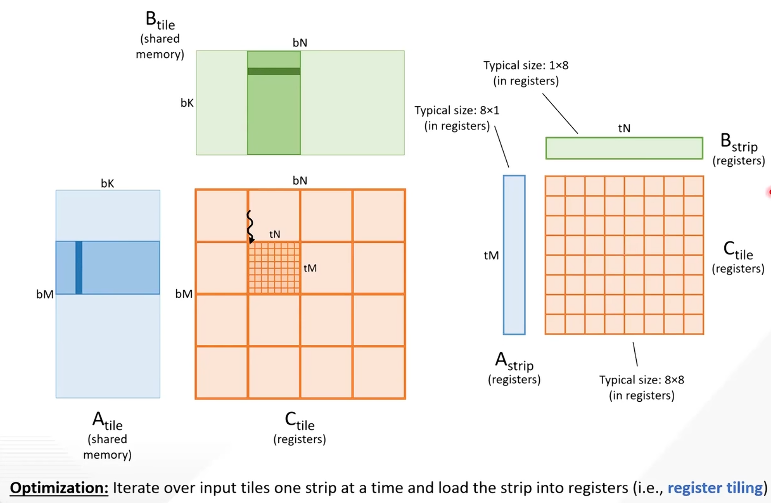
\includegraphics[width=0.8\textwidth]{images/image-25.png}
\caption{Register Tiling}
\end{figure}
\begin{figure}
\centering
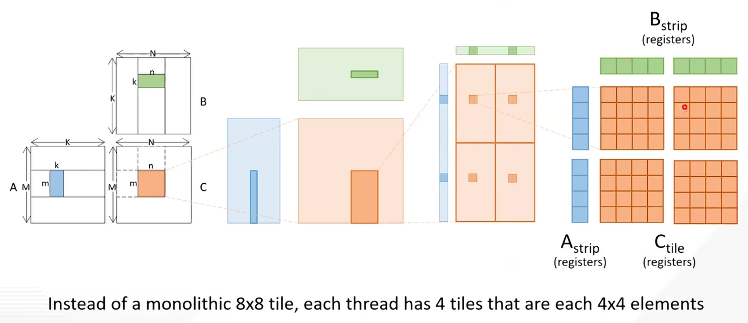
\includegraphics[width=0.8\textwidth]{images/image-26.png}
\caption{Rearranging Tiles to Coalesce Stores}
\end{figure}
\begin{figure}
\centering
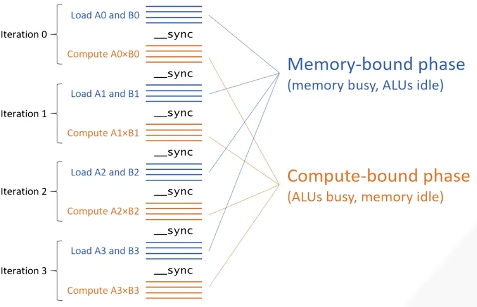
\includegraphics[width=0.8\textwidth]{images/image-27.png}
\caption{Motivation for Software Pipelining}
\end{figure}


\newpage

\end{document}
